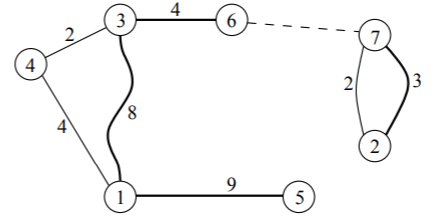
\includegraphics{islands.png}

$N = 7$ мостов в примере таковы: $(1-3)$, $(2-7)$, $(3-4)$, $(4-1)$, $(5-1)$,
$(6-3)$ и $(7-2)$. Заметьте, что два различных моста соединяют острова $2$ и
$7$.

Один из способов получить максимальное расстояние таков:

\begin{shortitems}
  \item Начать с острова $5$.
  \item Пройти по мосту длины $9$ и оказаться на острове $1$.
  \item Пройти по мосту длины $8$ и оказаться на острове $3$.
  \item Пройти по мосту длины $4$ и оказаться на острове $6$.
  \item Переправиться на пароме на остров $7$.
  \item Пройти по мосту длины $3$ и оказаться на острове $2$.
\end{shortitems}

В конце вы окажетесь на острове $2$ и суммарное расстояние будет равно
$9+8+4+3 = 24$. Единственный остров, оставшийся непосещённым, "--- $4$.
Заметьте, что по окончании описанного путешествия ни один остров больше
посетить нельзя. Более точно:

\begin{shortitems}
  \item Нельзя отправиться туда пешком, так как нет моста, соединяющего $2$
    (текущий остров) и $4$.
  \item Нельзя воспользоваться паромом, так как $4$ достижим из $2$, где вы
    теперь находитесь. Способ его достичь: воспользоваться мостом $(2-7)$,
    затем переправиться на пароме, которым вы уже переправлялись с острова
    $7$ на остров $6$, затем мост $(6-3)$ и, наконец, мост $(3-4)$.
\end{shortitems}
